% Source: originals/shrock-phy541/homework/phy541_hw2.pdf (typed handout dated Feb. 23, 2026). The "accompanying
% sheet" with the graphs is not among the scans; the graphs below are drawn from the descriptions in the problems.
% Placed after mean field theory; it uses Lectures 8-11.
\hwset{2}

\noindent\emph{Dated Feb.\ 23, 2026.} This homework assignment is due in class on Wed., Mar.\ 4. The total point value
is 170 points. To avoid cumbersome notation, we leave the subscript $P$ on $v_P$ implicit below, writing it simply as
$v$.

\begin{diagram}
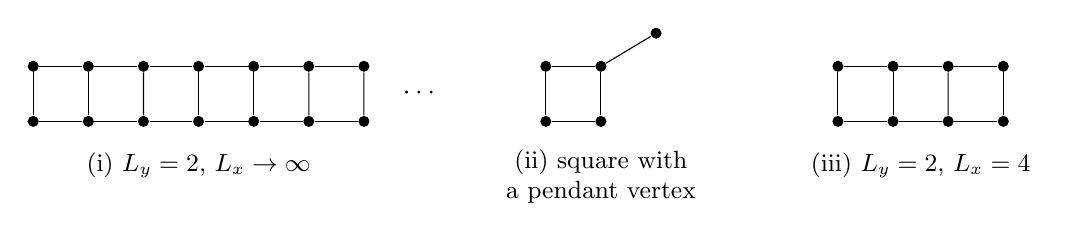
\begin{tikzpicture}[scale=0.7,gv/.style={circle,fill,inner sep=0pt,minimum size=4pt}]
  % (i) strip of the square lattice, width 2, long
  \foreach \x in {0,...,6} {\node[gv] (a\x) at (\x,0) {}; \node[gv] (b\x) at (\x,1) {}; \draw (a\x) -- (b\x);}
  \foreach \x [evaluate=\x as \y using int(\x+1)] in {0,...,5} {\draw (a\x) -- (a\y); \draw (b\x) -- (b\y);}
  \node at (7.0,0.5) {$\cdots$};
  \node[font=\small] at (3,-0.8) {(i) $L_y = 2$, $L_x\to\infty$};
  % (ii) square with a pendant vertex
  \begin{scope}[xshift=9.3cm]
    \node[gv] (s1) at (0,0) {}; \node[gv] (s2) at (1,0) {}; \node[gv] (s3) at (1,1) {}; \node[gv] (s4) at (0,1) {};
    \node[gv] (s5) at (2,1.6) {};
    \draw (s1) -- (s2) -- (s3) -- (s4) -- (s1); \draw (s3) -- (s5);
    \node[font=\small,align=center] at (1,-1.0) {(ii) square with\\ a pendant vertex};
  \end{scope}
  % (iii) ladder 2 x 4
  \begin{scope}[xshift=14.6cm]
    \foreach \x in {0,...,3} {\node[gv] (c\x) at (\x,0) {}; \node[gv] (d\x) at (\x,1) {}; \draw (c\x) -- (d\x);}
    \foreach \x [evaluate=\x as \y using int(\x+1)] in {0,...,2} {\draw (c\x) -- (c\y); \draw (d\x) -- (d\y);}
    \node[font=\small] at (1.5,-0.8) {(iii) $L_y = 2$, $L_x = 4$};
  \end{scope}
\end{tikzpicture}
\diagramcaption{The graphs of Problems 2.2 to 2.5, drawn from their descriptions (the accompanying sheet is not among
the scans).}\label{fig:hw2graphs}
\end{diagram}

\begin{hwproblem}{2}{1}
(30 pts) Consider the $q$-state Potts antiferromagnet with $q\ge 3$ on the infinite triangular lattice. (Formally, one
may define this lattice starting with a finite section of this lattice with free boundary conditions and taking the
thermodynamic limit.) Does this model obey the Third Law of Thermodynamics, that the entropy per vertex (= site),
$\bar S\to 0$ as the temperature $T\to 0$? How does your answer depend on $q$, if at all? Prove all of your
assertions.
\end{hwproblem}

\begin{hwproblem}{2}{2}
(20 pts) Consider the ferromagnetic zero-field spin-$1/2$ Ising model on a strip graph of the square lattice shown in
the accompanying sheet (Figure~\ref{fig:hw2graphs}(i)), with width $L_y = 2$ vertices and arbitrarily great length
$L_x$ vertices, with free transverse and longitudinal boundary conditions. Recall that the Hamiltonian for this model
is $\Ham = -J\sum_{\langle i,j\rangle}\sigma_i\sigma_j$, where $J>0$, $\langle i,j\rangle$ denote adjacent vertices, and
$\sigma_i = \pm1$. The following questions apply in the limit $L_x\to\infty$: (a, 10 pts) Calculate the mean-field
theory prediction for the critical temperature, $T_c$; (b, 10 pts) What is the actual critical temperature? Prove your
results.
\end{hwproblem}

\begin{hwproblem}{2}{3}
(50 pts) From the cluster expansion representation for the partition function of the Potts model on a graph $G$,
$Z(G,q,v)$, it follows that $Z(G,q,v) = Z(G-e,q,v)+vZ(G/e,q,v)$, in the notation used in class, where $e$ denotes an
edge in $G$ and $v\equiv v_P$. Consider a graph comprised of a square with an additional vertex joined to one of the
vertices of the square by a bond, as shown on the accompanying sheet (Figure~\ref{fig:hw2graphs}(ii)). Calculate (a, 20
pts) the chromatic polynomial, $P(G,q)$; (b, 20 pts), the Potts model partition function $Z(G,q,v)$; and (c, 10 pts)
the Tutte polynomial $T(G,x,y)$ for this graph. Here, as discussed in class, $x = 1+(q/v)$ and $y = v+1$.
\end{hwproblem}

\begin{hwproblem}{2}{4}
(30 pts) Consider the same graph as in the previous problem, namely a square with an additional vertex joined to one
of the vertices of the square by a bond. Calculate (a, 10 pts) the number of spanning trees, (b, 10 pts) the number of
spanning forests, (c, 10 pts) the number of connected spanning subgraphs.
\end{hwproblem}

\begin{hwproblem}{2}{5}
(20 pts) Consider a ladder graph of the square lattice with width $L_y = 2$ vertices and length $L_x = 4$ vertices,
with free transverse and longitudinal boundary conditions, as shown on the accompanying sheet
(Figure~\ref{fig:hw2graphs}(iii)). Calculate the total number of spanning subgraphs of this graph.
\end{hwproblem}

\begin{hwproblem}{2}{6}
(20 pts) Calculate the mean-field prediction for the critical temperature of a (zero-field) ferromagnetic $O(2)$ spin
model with spin-spin coupling $J$ on the hcp (hexagonal close packed) lattice.
\end{hwproblem}
